
%!TEX TS-program = xelatex
%----------------------------------------------------------------------------------------
%	PACKAGES AND THEMES
%----------------------------------------------------------------------------------------
\documentclass[aspectratio=169,xcolor=dvipsnames, t]{beamer}
\usepackage{fontspec}
\usepackage{unicode-math}
\setmathfont{latinmodern-math.otf}
\usetheme{SimplePlusAIC}
\usepackage{hyperref}
\usepackage{graphicx}
\usepackage{booktabs}
\usepackage{tikz}
\usepackage{makecell}
\usepackage{wrapfig}
\usepackage[spanish]{babel}
\usepackage[numbers]{natbib}
\usepackage{subcaption}

%----------------------------------------------------------------------------------------
%	TITLE PAGE CONFIGURATION
%----------------------------------------------------------------------------------------

\title[Pronóstico de Violencia Extrema]{Fortalecimiento del SAT mediante aprendizaje de máquinas en la detección de violencia atípica}
\subtitle{Economía y Derecho}

\author[Heredia Niño]{Juan Diego Heredia Niño}
\institute[Universidad de los Andes]{Facultad de Economía \newline Universidad de los Andes}

\date{\today} 

%----------------------------------------------------------------------------------------
%	PRESENTATION SLIDES
%----------------------------------------------------------------------------------------

\begin{document}

\maketitlepage

\begin{frame}{Enfoque Analítico del Estudio}
    \vspace{0.4cm}
\textbf{Perspectiva de violencia:} \alert{Seguridad pública}
        \pause
        \vspace{0.2cm}
        \begin{itemize}
            \item Incidencia de \alert{grupos armados} y \alert{criminales}:
            \begin{itemize}
                \item Economías ilícitas
                \item Control territorial
                \item Confrontación armada
            \end{itemize}
            
            \vspace{0.4cm}
            \pause
            \item Impacto de la violencia: 
            \begin{itemize}
                \item Vida cotidiana de la población
                \item Gobernanza local 
                \item Estabilidad institucional
            \end{itemize}
        \end{itemize}

\end{frame}

\makesection{Motivación}


\begin{frame}{Evolución de la Violencia en Colombia}
    \begin{figure}[ht]
        \centering
        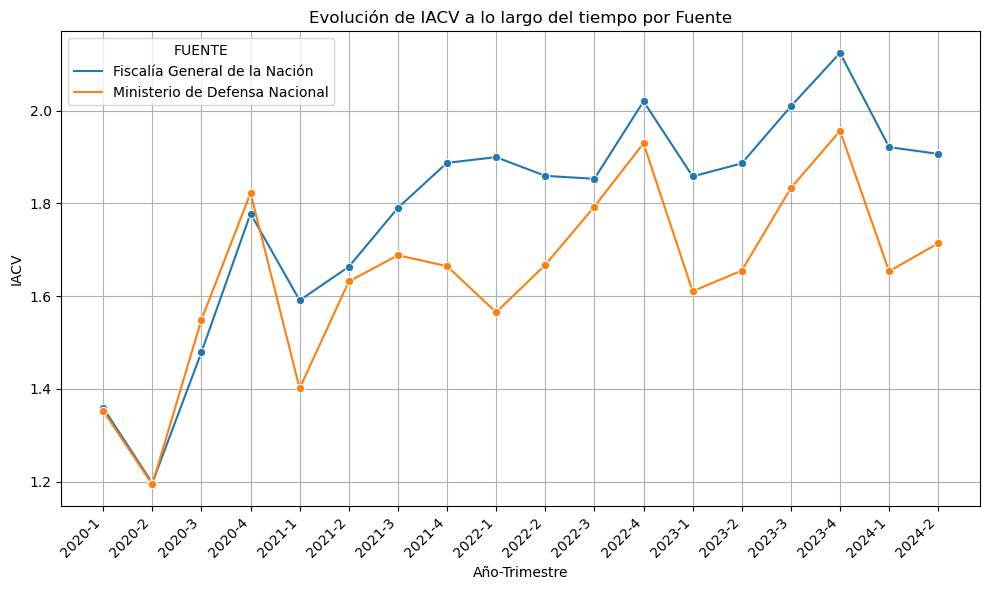
\includegraphics[width=0.9\textwidth, height=0.7\textheight, keepaspectratio]{images/image 7.png}
    \end{figure}
    \centering
    \footnotesize\textit{Fuente: Datos  MinDefensa. Elaboración propia}
\end{frame}

\begin{frame}{Vulnerabilidad municipal a la violencia}
    \begin{columns}[T]
        % Columna izquierda
        \begin{column}{0.48\textwidth}
            \centering
            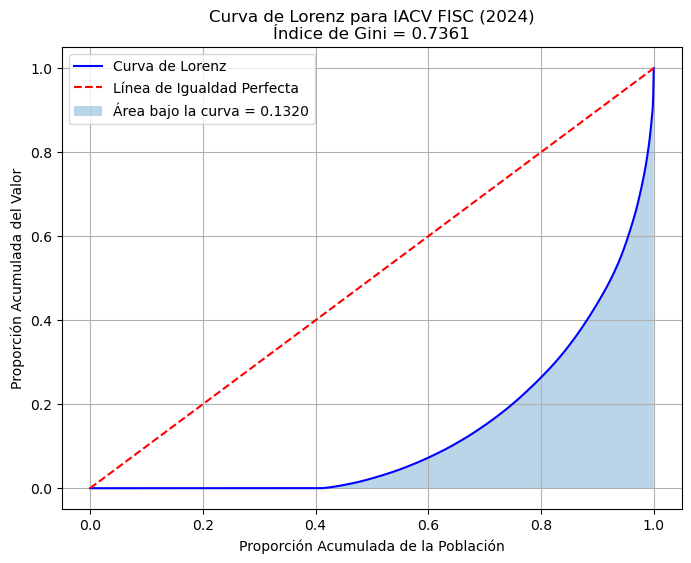
\includegraphics[width=\textwidth, height=0.65\textheight, keepaspectratio]{images/image 4.png}
        \end{column}
        
        % Columna derecha
        \begin{column}{0.48\textwidth}
            \centering
            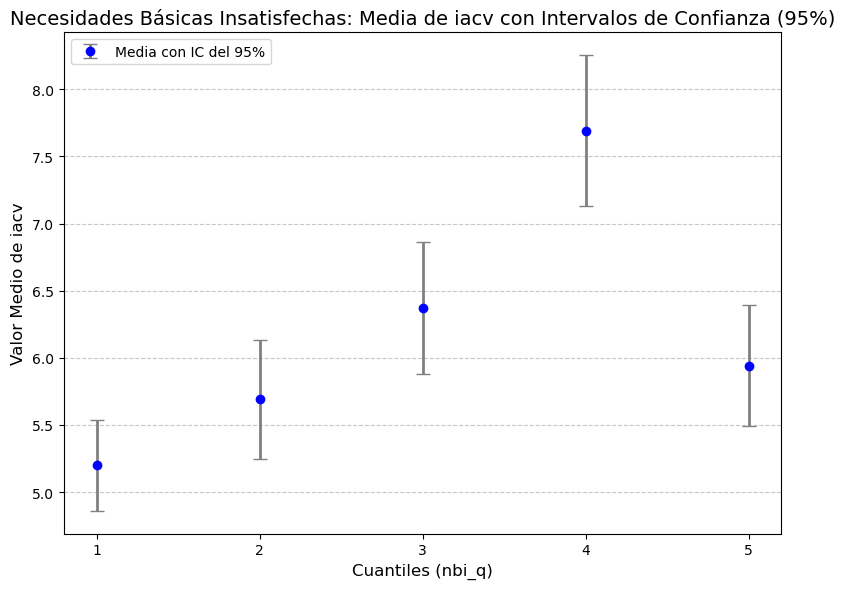
\includegraphics[width=\textwidth, height=0.65\textheight, keepaspectratio]{images/output1.png}
        \end{column}
    \end{columns}
    \vspace{0.2cm}
    \centering
    \footnotesize\textit{Fuente: Datos Panel CEDE y MinDefensa. Elaboración propia}
\end{frame}



\begin{frame}{Motivación}
    \small
    \begin{block}{¿Por qué importa esta pregunta?}
        \begin{itemize}
            \item La violencia atípica tiene \textbf{alto impacto social} y \textbf{poca capacidad de respuesta}.
            \item Las herramientas actuales (SAT) son cualitativas y pueden no detectar patrones emergentes.
        \end{itemize}
    \end{block}
    
    \begin{block}{¿Qué propone esta tesis?}
        \begin{itemize}
            \item Usar \textbf{aprendizaje automático} para predecir eventos críticos.
            \item Complementar el SAT con una herramienta cuantitativa y replicable.
        \end{itemize}
    \end{block}

%    \begin{block}{¿Por qué ahora?}
%        \begin{itemize}
%            \item Mayor disponibilidad de datos detallados sobre violencia y contexto municipal.
%            \item Necesidad urgente de mejorar la prevención frente a conflictos armados y crimen organizado.
%        \end{itemize}
%    \end{block}
\end{frame}

%\begin{frame}{Motivación}
%    \small
%    \begin{itemize}
%        \item La violencia atípica genera altos costos sociales, económicos y humanitarios, especialmente cuando se presenta de forma repentina e intensa, dejando poco tiempo de respuesta institucional.
        
%        \vspace{0.35cm}
%        \item El Sistema de Alertas Tempranas (SAT) ha sido clave para prevenir violaciones a los derechos humanos, pero se basa en metodologías cualitativas que pueden no ser tan rápidas, ni tomar en cuenta patrones no observables.
        
%        \vspace{0.35cm}
%        \item Integrar herramientas de aprendizaje automático permite \textbf{identificar con anticipación eventos atípicos de violencia} apoyando la capacidad de reacción del Estado.
        
%        \vspace{0.35cm}
%        \item Esta tesis busca ofrecer una herramienta cuantitativa que complemente el SAT y \textbf{fortalezca la prevención basada en evidencia}.
%    \end{itemize}
%\end{frame}
\makesection{Resultados preliminares}

\begin{frame}{¿Ayuda el aprendizaje automático?}
    \small
    \begin{block}{Hallazgo principal (preliminar)}
        Los modelos de aprendizaje automático \textbf{mejoran la capacidad de detección de violencia atípica} frente a métodos tradicionales:
        \begin{itemize}
            \item \textbf{Mayor precisión global} (hasta 85.4\% con Random Forest).
            \item \textbf{Mejor equilibrio} entre sensibilidad y precisión (\textit{F1} $\approx$ 0.75).
            \item \textbf{AUC elevado} ($\approx$ 0.89), lo que permite \textbf{priorizar municipios según su riesgo estimado}, abriendo la puerta a un sistema de alerta más focalizado y preventivo.
        \end{itemize}
    \end{block}

    \vspace{0.2cm}
    \begin{block}{Advertencia}
        Estos resultados son \textbf{preliminares} y están sujetos a revisión en etapas posteriores.
    \end{block}
\end{frame}
\input{sections/revisión de literatura.tex}

\makesection{Definiciones}

\begin{frame}[label=iacv]{Índices de Violencia}
    \textbf{Índice de Violencia Agregada (IACV)}
    \begin{itemize}
        \item Suma ponderada de homicidio, extorsión, secuestro, terrorismo y masacres.
        \item Ponderado según la pena promedio del delito según el Código Penal Colombiano.
    \end{itemize}

    \begin{table}[]
        \centering
        \begin{tabular}{@{}lcc@{}}
        \toprule
        Delito & Pena Promedio (Años) & Porcentaje Relativo (\%) \\ \midrule
        Homicidio & 19.0 & 17.04 \\
        Extorsión & 11.5 & 10.31 \\
        Secuestro & 16.0 & 14.35 \\
        Terrorismo & 15.0 & 13.45 \\
        Masacres & 50.0 & 44.84 \\ \bottomrule
        \end{tabular}
        \caption{Penas promedio por delito y su ponderación}
    \end{table}
\end{frame}

\begin{frame}[label=violencia_atipica]{Violencia Extrema o Atípica}
    \begin{itemize}
        \item Se utiliza un umbral basado en la desviación estándar del índice de violencia.
        \item Eventos cercanos a la media se consideran normales.
        \item Eventos alejados (e.g., +1.5σ o +2σ) se interpretan como atípicos o críticos.
    \end{itemize}
\end{frame}


\makesection{Datos}
\begin{frame}{Fuentes de Datos}
Los datos de violencia provienen de tres fuentes principales:

\begin{itemize}
    \item \textbf{Fiscalía General de la Nación}: Registros mensuales de \alert{homicidio, extorsión, secuestro, terrorismo y masacres} a nivel municipal, mensual (2014-2024).
    \item \textbf{Ministerio de Defensa Nacional}: Serie histórica de los mismos delitos con \alert{mayor cobertura temporal} a nivel municipal, mensual(1997-2024)%, permitiendo análisis de tendencias a largo plazo. Idea para hacer PCA para los datos antes del corte de la fiscalía
    \item \textbf{Jurisdicción Especial para la Paz (JEP)}: Datos sobre \alert{presencia de grupos armados y eventos violentos} (2017-2024), incluyendo desplazamientos, hostigamientos y paros armados.
\end{itemize}
\end{frame}
\begin{frame}{Fuentes de Datos}

Para analizar la relación entre violencia y factores estructurales, se integran:

\begin{itemize}
    \item \textbf{Panel Municipal del CEDE} (2005-2023): Información demográfica, socioeconómica e institucional, como \alert{pobreza, acceso a servicios y programas para víctimas}.
    \item \textbf{Cultivos ilícitos de coca} (1999-2023, Observatorio de Drogas de Colombia): Financiación de grupos armados y la \alert{dinámica del conflicto}.
    \item \textbf{Luminosidad nocturna (VIIRS Nighttime Light)} (2012-2023): Indicador proxy de \alert{actividad económica local}.
\end{itemize}
\end{frame}

\makesection{Metodología}

\begin{frame}{Modelo Teórico: Clasificación Binaria}

    \begin{itemize}
        \item \alert{Aprendizaje Supervisado}: \textbf{Clasificación Binaria}
        $$y = f(X)$$
        \pause
        \item \textbf{Función de probabilidad}:
        \[
        y_t = \begin{cases} 
            1 & \text{si } \text{IACV}_t \geq \bar{X} + \sigma \text{ (atípico)} \\
            0 & \text{si } \text{IACV}_t < \bar{X} + \sigma \text{ (normal)}
        \end{cases}
        \]
        \end{itemize}
\end{frame}





\begin{frame}{Estimación}
    \begin{alertblock}{Objetivo}
        Estimar \( P(y=1|X) \) para activar alertas tempranas con \( \uparrow \) precisión y \( \uparrow \) sensibilidad
    \end{alertblock}
    \pause
    \begin{itemize}
        \item \textbf{Variables explicativas \( X \)}:
        \pause
        \begin{itemize}
            \item \alert{Factores estructurales}:
            \begin{itemize}
                \footnotesize
                \item Desigualdad, presencia estatal, economías ilegales, empleo, presencia grupos armados, educación, ubicación, etc.
            \end{itemize}
            \pause
            \item \alert{Rezagos temporales de violencia}:
            \begin{itemize}
                \footnotesize
                \item IACV, IGC e IA
            \end{itemize}
        
        \end{itemize}
        \end{itemize}
\end{frame}




\begin{frame}{Enfoques de Machine Learning: Elastic Net y Random Forest}
    \begin{columns}[T]
        \begin{column}{0.48\textwidth}
            \begin{alertblock}{1. Elastic Net}
                \begin{itemize}
                    
                    \item \textbf{Qué hace}: 
                    \begin{itemize}
                        
                        \item Regresión lineal con penalización combinada L1 (Lasso) y L2 (Ridge)
                    \end{itemize}
                    \item \textbf{Ventaja}: 
                    \begin{itemize}
                        
                        \item Selección automática de variables y reducción de sobreajuste
                    \end{itemize}
                \end{itemize}
            \end{alertblock}
        \end{column}
        
        \begin{column}{0.48\textwidth}
            \begin{alertblock}{2. Random Forest}
                \begin{itemize}
                    
                    \item \textbf{Qué hace}: 
                    \begin{itemize}
                        
                        \item Ensamble de múltiples árboles de decisión
                    \end{itemize}
                    \item \textbf{Ventaja}: 
                    \begin{itemize}
                        
                        \item Maneja alta dimensionalidad y reduce el sobreajuste
                    \end{itemize}
                \end{itemize}
            \end{alertblock}
        \end{column}
    \end{columns}
\end{frame}

\begin{frame}{Enfoques de Machine Learning: XGBoost y LSTM}
    \begin{columns}[T]
        \begin{column}{0.48\textwidth}
            \begin{alertblock}{3. XGBoost}
                \begin{itemize}
                    
                    \item \textbf{Qué hace}: 
                    \begin{itemize}
                        
                        \item Boosting con n iteraciones + regularización
                    \end{itemize}
                    \item \textbf{Ventaja}: 
                    \begin{itemize}
                        \item Similar a Random Forest
                        \item Eficiencia con datos desbalanceados
                        \item Tratamiento de valores nulos
                    \end{itemize}
                \end{itemize}
            \end{alertblock}
        \end{column}
        
        \begin{column}{0.48\textwidth}
            \begin{alertblock}{4. Redes LSTM}
                \begin{itemize}
                    
                    \item \textbf{Qué hace}: 
                    \begin{itemize}
                        
                        \item Modela dinámicas temporales de forma más efectiva que métodos tradicionales
                    \end{itemize}
                    \item \textbf{Ventaja}: 
                    \begin{itemize}
                        
                        \item Detecta patrones temporales críticos 
                    \end{itemize}
                \end{itemize}
            \end{alertblock}
        \end{column}
    \end{columns}

\end{frame}


\begin{frame}{}
    \vspace{3.5cm}
    \centering
    \LARGE \alert{\textbf{¡Gracias!}} 

\end{frame}

\begin{frame}{Referencias}

\begin{itemize}
\tiny
    \item Banco Interamericano de Desarrollo. (2017). \textit{Los costos del crimen y la violencia}. Banco Interamericano de Desarrollo. \url{https://doi.org/10.18235/0006383}

    \item Bazzi, S., Blair, R. A., Dube, O., Gudgeon, M., \& Peck, R. (2022). \textit{The promise and pitfalls of conflict prediction: Evidence from Colombia and Indonesia}. \textit{The Review of Economics and Statistics, 104} (6), 1246–1262. \url{https://doi.org/10.1162/rest_a_01172}
    
    \item Bourguignon, F., Núñez, J., \& Sánchez, F. (2003). \textit{What part of the income distribution does inequality affect crime? The case of Colombia}. Documento CEDE, Universidad de los Andes.

    \item Dube, O., \& Vargas, J. F. (2013). \textit{Commodity price shocks and civil conflict: Evidence from Colombia}. \textit{Review of Economic Studies, 80}(4), 1384–1421. \url{https://doi.org/10.1093/restud/rdt009}

    \item Feldmann, A., \& Hinojosa, V. (2009). \textit{Terrorism in Colombia: Logic and sources of a multidimensional and ubiquitous phenomenon}. \textit{Terrorism and Political Violence, 21} (1), 42-61. \url{https://doi.org/10.1080/09546550802544694}

    \item Levitt, S., \& Rubio, M. (2000). \textit{Understanding crime in Colombia and what can be done about it}. Documento de trabajo, Universidad de Chicago/Fedesarrollo.

    \item Londoño, J. L., \& Guerrero, R. (1999). \textit{Violencia en América Latina: Epidemiología y costos}. Banco Interamericano de Desarrollo.

    \item Mejía, D., \& Restrepo, P. (2011). \textit{The economics of the war on illegal drug production and trafficking}. Documento CEDE, Universidad de los Andes.

    \item Rubio, M. (2003). \textit{El rapto de la pesca milagrosa: Breve historia del secuestro en Colombia}. Documentos CEDE No. 2003-36, Universidad de los Andes.

    \item Sánchez, F., \& Chacón, M. (2005). \textit{Conflicto, Estado y descentralización: Disputa armada por el control local, 1974–2002}. Documento CIDER/Universidad de los Andes – LSE.

\end{itemize}
\end{frame}

\end{document}
